The aim of this exercise is generating pseudo random numbers by a computer algorithm such that the output is a sequence of reals
or integers, which suppose to be uniformly distributed on $[0,1]$ and statistically independent.
\subsection{Linear Congruential Generator (LCG)}
In the first step of this exercise, Linear Congruential Generator (LCG) is implemented for generating $10000$ random numbers by
\begin{equation}
    x_i=mod(ax_{i-1}+c, M),              U_i=\frac{x_i}{M}
\end{equation}
Where a is a multiplier, c is a shift and M is modulus, then these numbers is presented by a histogram for 10 classes.
\begin{center}
    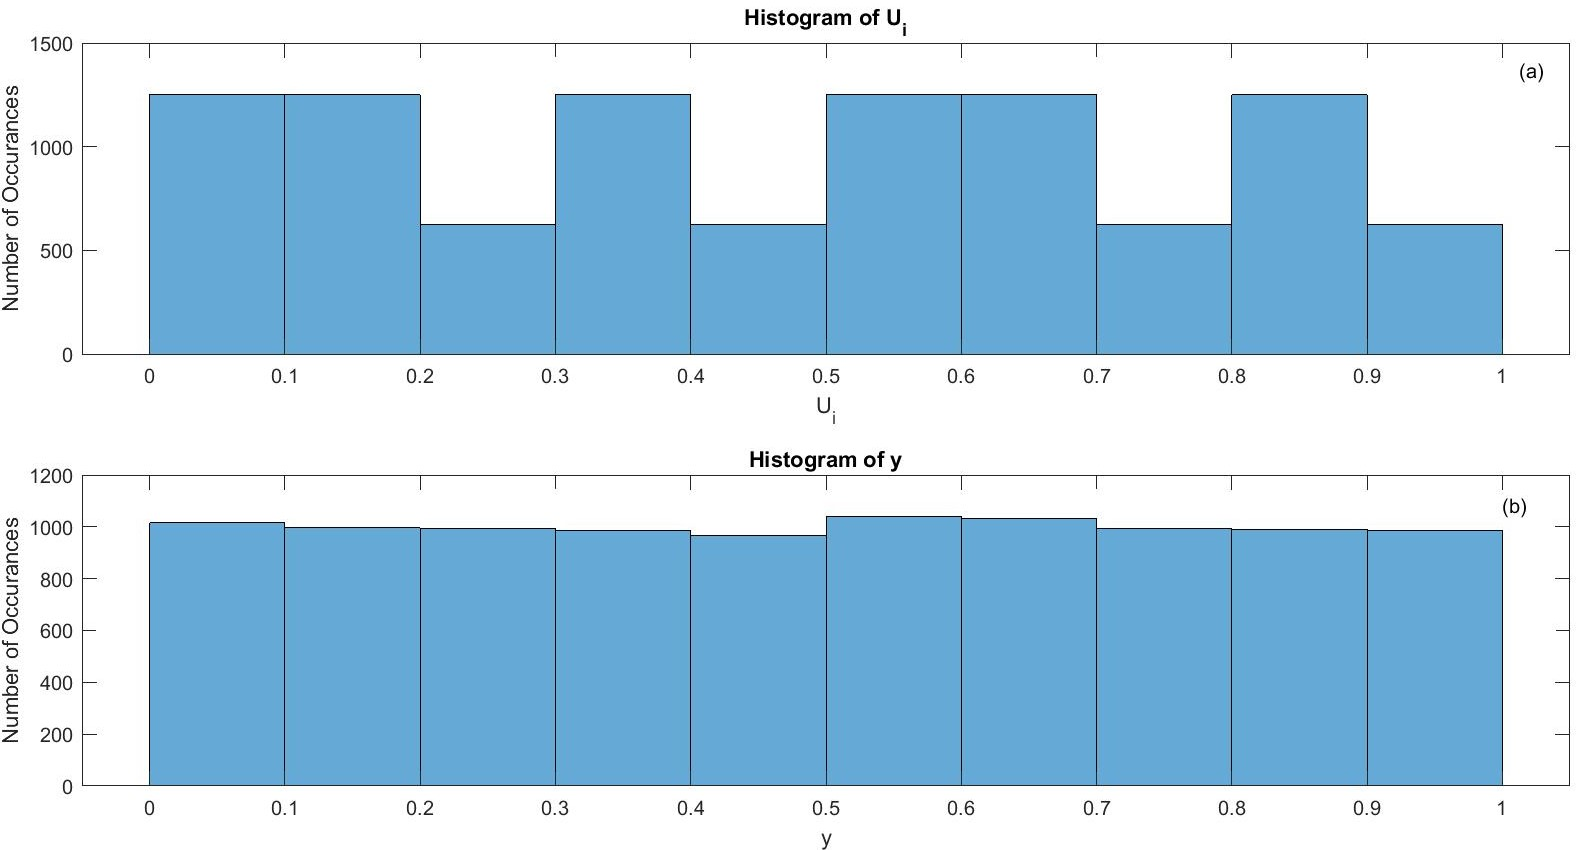
\includegraphics[scale=0.3]{Figures/figure1_1.jpg}\\
    \figuretitle{Figure 1: Histogram for U and Y.}
\end{center}\\
\\
Figure 1 show the histogram for U which generated by LCG and the histogram for Uniformly distributed random numbers.\\
\subsection{Evaluate the quality of the generators}
 The quality of the generators is evaluated  by graphical descriptive statistics (histogrammes, scatter plots) and statistical tests ($X^2$,Kolmogorov-Smirnov, run-tests, and correlation test).\\
 \begin{center}
    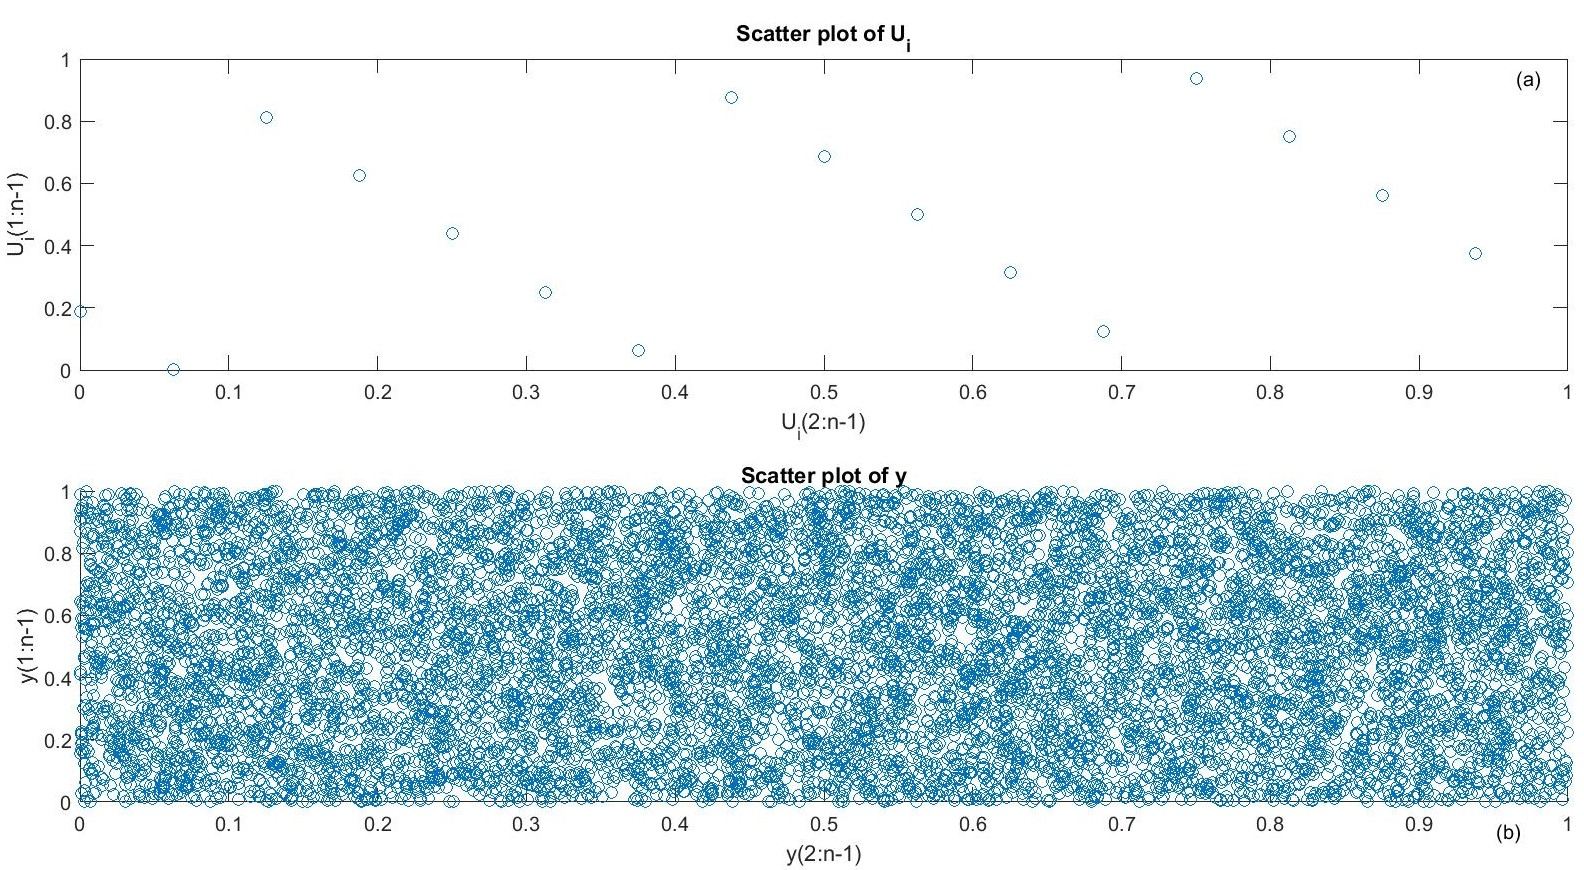
\includegraphics[scale=0.3]{Figures/figure1_2.jpg}\\
    \figuretitle{Figure 2: Scatter plot for U and Y.}
\end{center}\\
\\In this part of exercise, A chi-squared test ($\chi^2$ test) as a  statistical hypothesis test is implemented that is given by
\begin{equation}
  T=  \Sigma^{i=1}_{n_{classes}} =\frac{(n_{observed,i}-n_{expected,i})^2}{n_{expected,i}}
\end{equation}
The chi-squared test is used for the randomness of data to determine whether there is a significant difference between the expected frequencies and the observed frequencies in one or more categories.A chi-squared test can be used to attempt rejection of the null hypothesis that the data are independent.\\
%\lstinputlisting[language=matlab]{chi2test.m}
\\Now for testing the type of distribution of the random number generator, we implemented Kolmogorov-Smirnov test that can be used to compare a sample with a reference probability distribution. In this respect, the Kolmogorov–Smirnov statistic compares empirical distribution function $F_{n}(x)$  with hypothesized distribution $F(x)$ and it quantifies a distance that is given by
\begin{equation}
    D_n=sup_{x}{|F_{n}(x)-F(x)|}
\end{equation}
 \begin{center}
    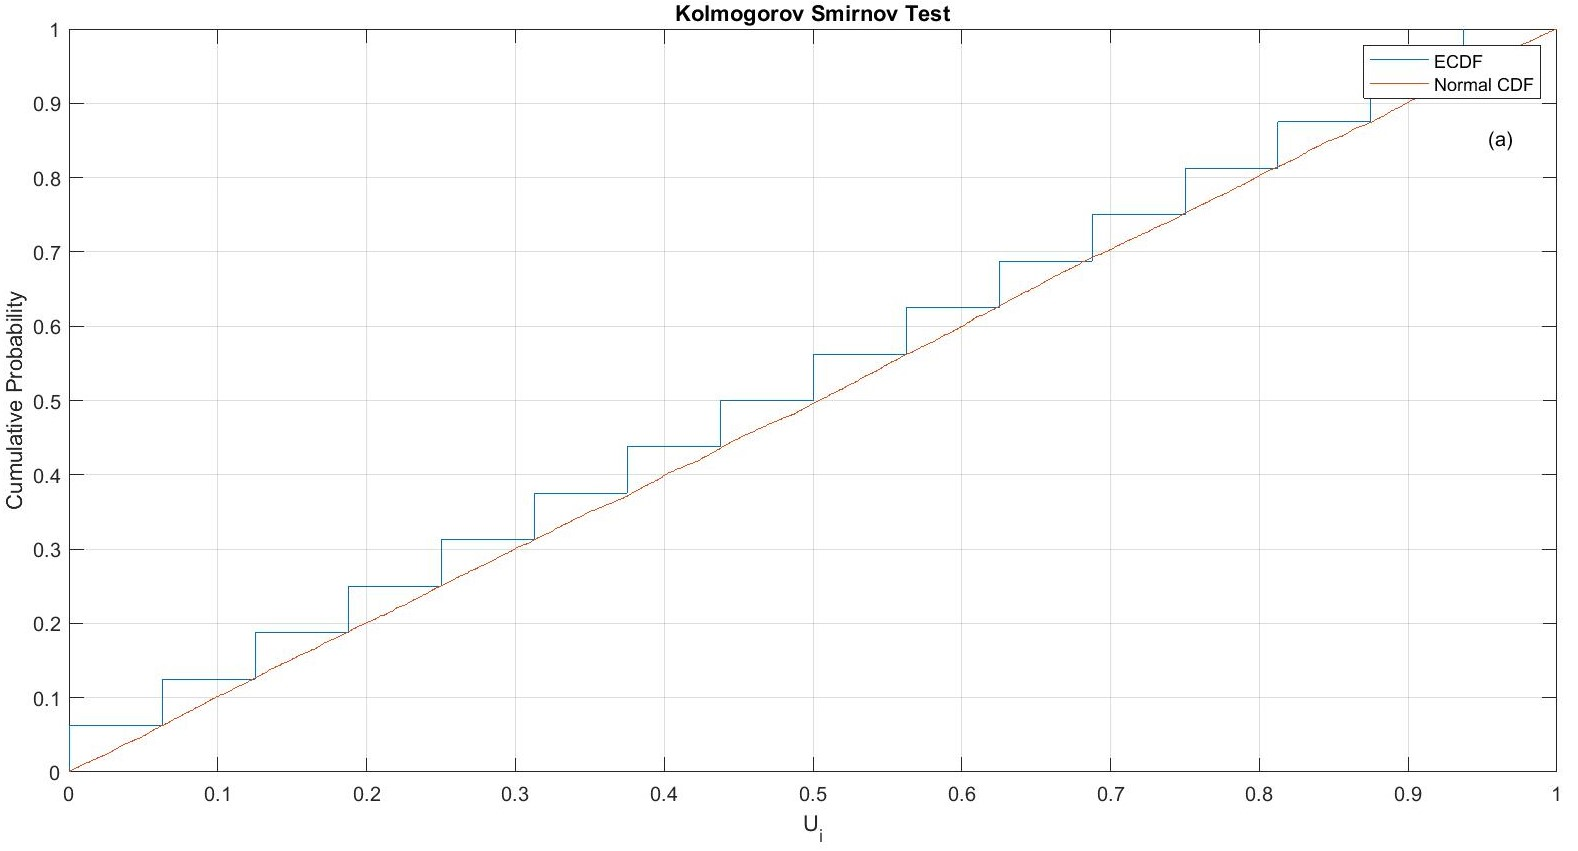
\includegraphics[scale=0.3]{Figures/figure1_3.jpg}\\
    \figuretitle{Figure 3: Kolmogorov–Smirnov Test .}
\end{center}\\
Figure 3 shows the Kolmogorov–Smirnov (KS) test.\\
Run test is other test which examines the arrangement of numbers in a sequence to test the hypothesis of independence and it can be used by comparing with the median.Let $n_1$ and $n_2$ be the number of individual observations above and below the mean, let b the total number of runs then the mean and variance of b can be expressed as 
\begin{equation}
    \mu_{b}=\frac{2n_{1}n_{2}}{2n_{1}+n_{2}}+1
\end{equation}
\begin{equation}
    \sigma^2_{b}=\frac{2n_{1}n_{2}(2n_{1}n_{2}-n_{1}-n_{2}}{(n_{1}+n_{2})^2(n_{1}+n_{2}-1)}
\end{equation}
$b$ is approximately normally distributed .\\
Correlation test is another independence test is given by
\begin{equation}
    C_{h}=\frac{1}{n-h}\Sigma^{i=1}_{n-h}U_{i}U_{i+h}\sim N(0.25,\frac{7}{144n})
\end{equation}





